\documentclass[11pt,letterpaper]{article}
\usepackage[lmargin=1in,rmargin=1in,tmargin=1in,bmargin=1in]{geometry}
\usepackage{../style/homework}
\usepackage{../style/commands}
\setbool{quotetype}{false} % True: Side; False: Under
\setbool{hideans}{false} % Student: True; Instructor: False

% -------------------
% Content
% -------------------
\begin{document}

\homework{17: Due 11/23}{I was on the street. This guy waved to me, and he came up to me and said, `I'm sorry. I thought you were someone else.' And I said, `I am.'}{Demetri Martin}

% Problem 1
\problem{10} Sketch the function $y= \log_2 x$. 
	\[
	\fbox{
	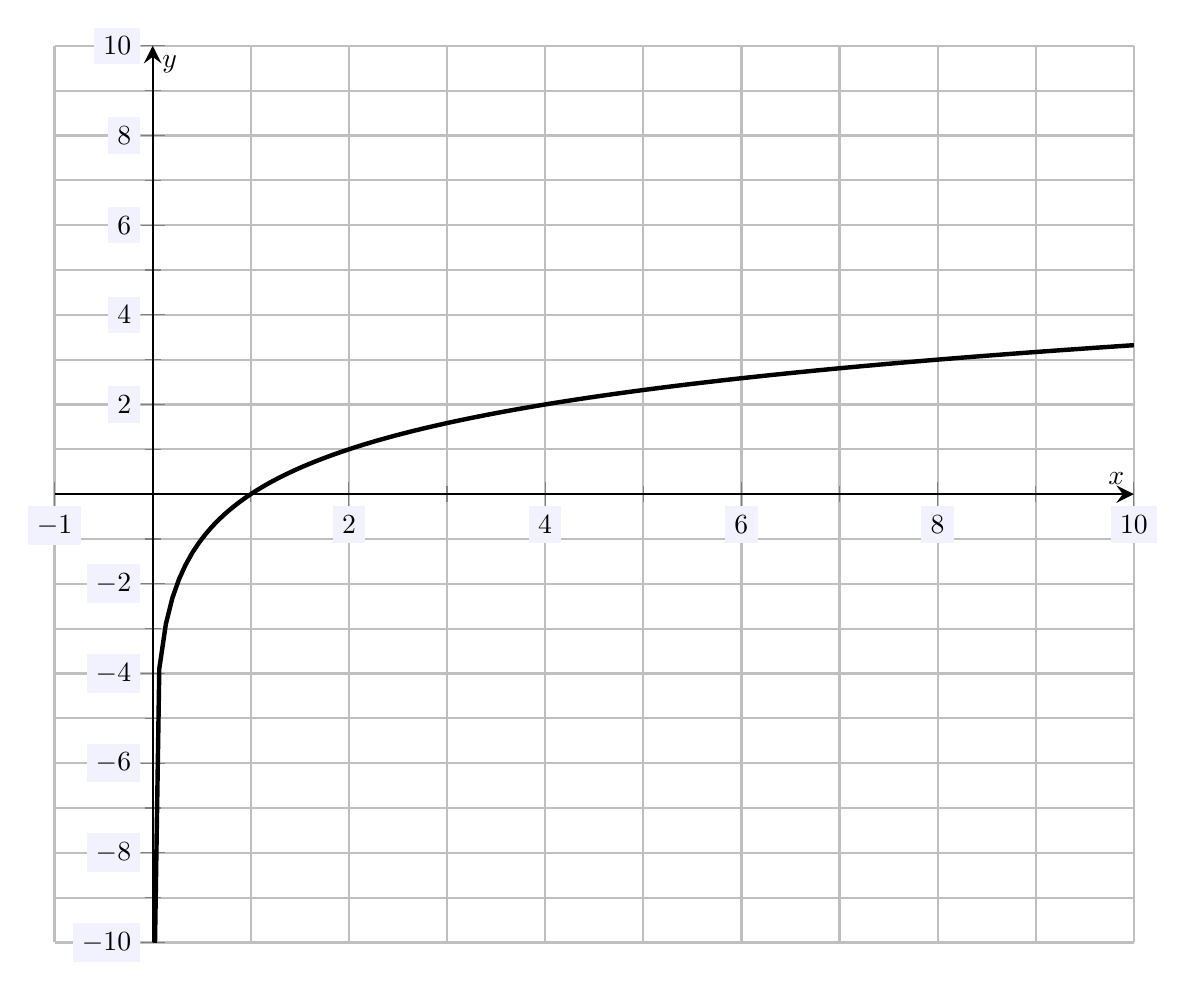
\begin{tikzpicture}[scale=2,every node/.style={scale=0.5}]
	\begin{axis}[
	grid=both,
	axis lines=middle,
	ticklabel style={fill=blue!5!white},
	xmin= -1, xmax=10,
	ymin= -10, ymax=10,
	xtick={-1,0,2,4,6,8,10},
	ytick={-10,-8,...,10},
	minor tick = {-10,-9,...,10},
	xlabel=\(x\),ylabel=\(y\),
	]
	\addplot[thick, domain= 0.0001:10,samples=150] {log2(x)};
	\draw[fill=black] (-2,1/64) circle (0.1);
	\end{axis}
	\end{tikzpicture}
	}
	\] \pspace





\newpage





% Problem 2
\problem{10} Compute the following:
\begin{enumerate}[(a)]
\item $\log_4 4 - \log_6 1$
\item $\log_5 25$
\item $\log_3 \dfrac{1}{81}$
\item $\log_9 \sqrt{3}$
\item $\ln e^{2/3}$
\end{enumerate} \pspace

\sol
\begin{enumerate}[(a)]
\item 
	\[
	\log_4 4 - \log_6 1= 1 - 0= 1
	\] \pspace

\item 
	\[
	\log_5 25= \log_5 5^2= 2
	\] \pspace

\item 
	\[
	\log_3 \dfrac{1}{81}= \log_3(81^{-1})= \log_3\big( (3^4)^{-1} \big)= \log_3(3^{-4})= -4
	\] \pspace

\item 
	\[
	\log_9 \sqrt{3}= \log_9(3^{1/2})= \log_9\big( (9^{1/2})^{1/2} \big)= \log_9(9^{1/4})= \dfrac{1}{4}
	\] \pspace

\item 
	\[
	\ln e^{2/3}= \log_e e^{2/3}= \dfrac{2}{3}
	\]
\end{enumerate}





\newpage 





% Problem 3
\problem{10} Expand the following logarithm completely by expressing it as a sum or difference of logs. Your answer should not include any exponents.
	\[
	\log_3 \left(\dfrac{\sqrt[6]{x}}{3y^4}\right)
	\] \pspace

\sol
	\[
	\begin{aligned}
	\log_3 \left(\dfrac{\sqrt[6]{x}}{3y^4}\right)&= \log_3 \sqrt[6]{x} - \log_3(3y^4) \\[0.3cm]
	&= \log_3 x^{1/6} - \log_3 y^4 - \log_3 3 \\[0.3cm]
	&= \frac{1}{6}\, \log_3 x - 4 \log_3 y - 1
	\end{aligned}
	\]





\newpage





% Problem 4
\problem{10} Rewrite the expression below as a single logarithm. 
	\[
	\frac{1}{2} \ln x - \ln 1 + 3\ln(x+2) - \ln(1 - x)
	\] \pspace

\sol
	\[
	\begin{aligned}
	\frac{1}{2} \ln x - \ln 1 + 3\ln(x+2) - \ln(1 - x)&= \ln x^{1/2} - 0 + \ln(x + 2)^3 - \ln(1 - x) \\[0.3cm]
	&= \ln \sqrt{x} + \ln\left( \dfrac{(x + 2)^3}{1 - x} \right) \\[0.3cm]
	&= \ln\left( \dfrac{\sqrt{x} (x + 2)^3}{1 - x} \right)
	\end{aligned}
	\]


%\printpoints
\end{document}